\newcommand{\rarr}{$\rightarrow$}

\chapter{Settings summary}
\begin{table}[htb]
	\centering
	\begin{tabular}{|l|c|}
		\hline
		\textbf{Parameter}	&	\textbf{Value}\\\hline\hline
		Serial port	&	individual (i.e. \textit{COM0} or \textit{/dev/ttyUSB0})\\\hline
		Command language	& HPGL\\\hline
		Resolution X	& 1000,0\\\hline
		Resolution Y	& 1000,0\\\hline
		Pen number		& 0\\\hline
		Pen force		& ignored\\\hline
		Pen speed		& ignored\\\hline
		Rotation		& 90°\\\hline
		Overcut			& 0,5-1,0 mm\\\hline
		Tool offset correction	& 0,25 mm\\\hline
		Auto align		& see \autoref{cha:extension}\\\hline
	\end{tabular}
	\caption{Inkscape export settings}
\end{table}

\begin{table}[htb]
	\centering
	\begin{tabular}{|l|c|}
		\hline
		\textbf{Parameter}	&	\textbf{Value}\\\hline\hline
		Speed		& 25 mm/s recommended, more possible\\\hline
		Force		& 75 g\\\hline
	\end{tabular}
	\caption{Plotter hardware setup}
\end{table}

{\let\clearpage\relax \chapter{Preparing your data}}
\begin{enumerate}
	\item Select everything: \textit{Edit} \rarr\ \textit{Select All} (\textit{ctrl}+\textit{a})
	\item Ungroup everything: \textit{shift}+\textit{ctrl}+\textit{g}, repeat until all groups are dissolved.
	\item Convert all objects to paths: \textit{Path} \rarr\ \textit{Object to Path} (\textit{shift}+\textit{ctrl}+\textit{c})
	\item If there are combined paths, break them apart: \textit{Path} \rarr\ \textit{Break Apart} (\textit{shift}+\textit{ctrl}+\textit{k})
	\item Rearrange the object order:
		\begin{itemize}
			\item \textit{Object} \rarr\ \textit{Objects...}
			\item Select the objects in the list to identify them. You can skip through the list fast using the arrow keys.
			\item The plotter will cut the objects in the order seen here. Change the order to minimize the required movements from one object to another.
		\end{itemize}
	\item optionally: Resize the page to your objects: \textit{Edit} \rarr\ \textit{Select All} (\textit{ctrl}+\textit{a}), \textit{Edit} \rarr\ \textit{Resize Page to Selection} (\textit{shift}+\textit{ctrl}+\textit{r})
\end{enumerate}

{\let\clearpage\relax \chapter{Setting up the plotter}}
\paragraph{Inserting the material}
\begin{enumerate}
	\item Move up the levers at the back of the plotter if not already.
	\item Insert the material.
	\item Slide the two rolls, that press down the material, so they both are above the material. You can grab them by the levers at the back side.
	\item Align the material.
	\item Push down the two levers to lock the position of the material.
\end{enumerate}

\begin{figure}[htb]
\centering
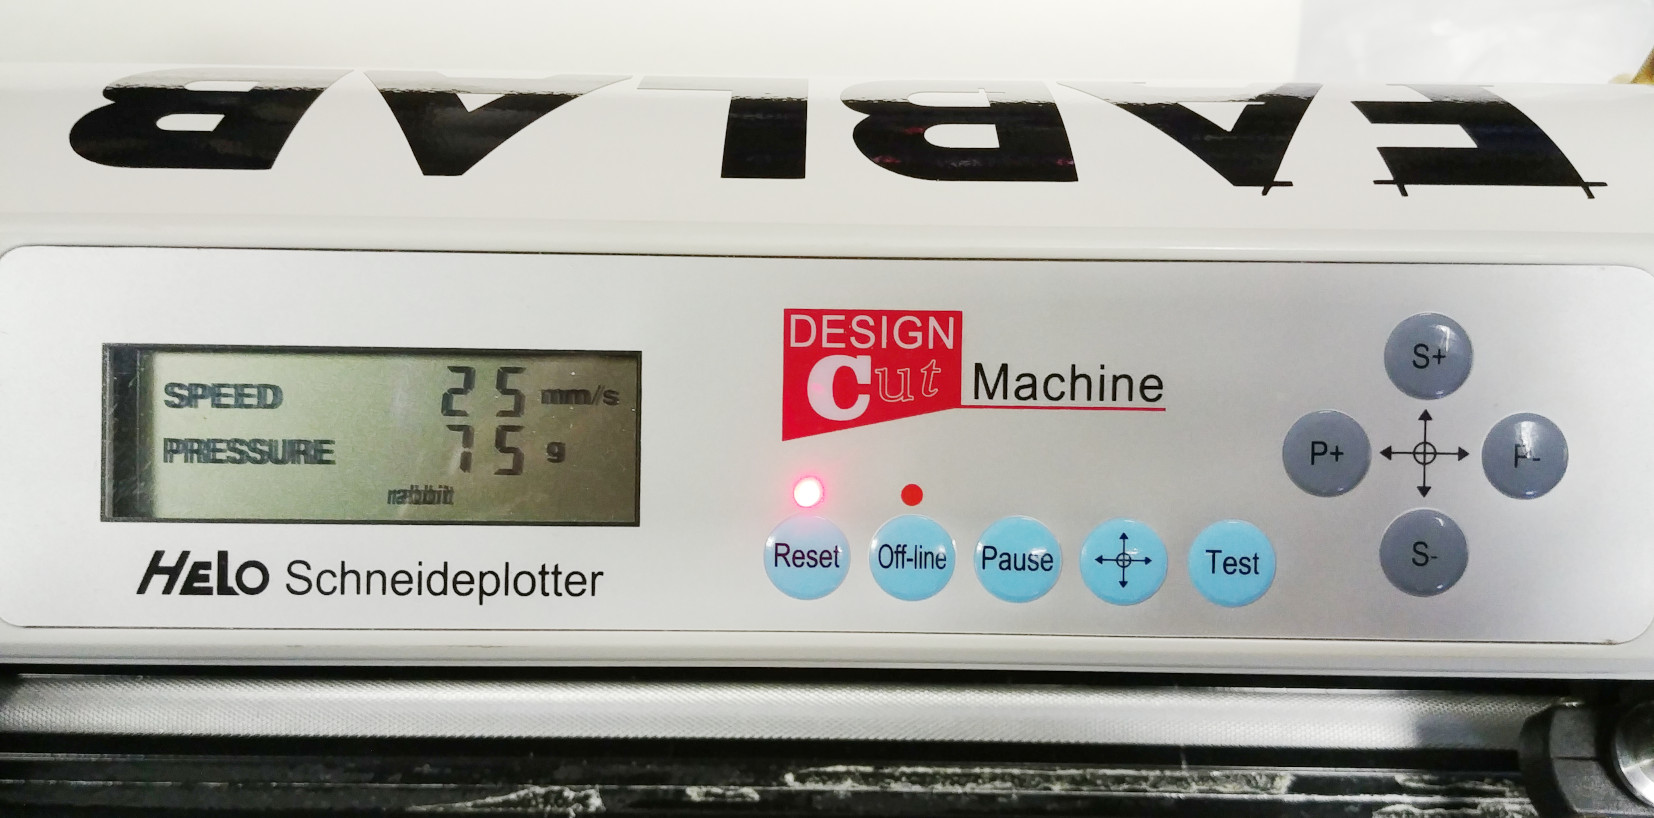
\includegraphics[width=0.8\textwidth]{images/plotter}
\caption{Interface of the plotter}
\label{fig:interface}
\end{figure}

\paragraph{Plotter settings}
\begin{enumerate}
	\item Set the speed with the \textit{S+}/\textit{S-} buttons. \SI{25}{\milli\meter\per\second} gives the best results, but faster settings may work, too.
	\item Set the pressure to \SI{75}{\gram} with the \textit{P+}/\textit{P-} buttons. This is the optimal value for \textit{Oracal 751C} (the foil available at \textsc{FabLab} Darmstadt). Other materials may require different values.
	\item Set the desired origin for cutting. The origin will be the lower right corner of your object or page:
	\begin{itemize}
		\item Press \textit{Off-line}
		\item Use the \textit{P} and \textit{S} buttons to move the knife to a the new origin.
		\item Press the ‚crossed arrows‘ button to confirm. This will exit the offline mode.		
	\end{itemize}
\end{enumerate}


{\let\clearpage\relax \chapter{Setting up the plotting extension in Inkscape}
\label{cha:extension}}
\begin{enumerate}
	\item Open the plotting extension: \textit{Extensions} \rarr\ \textit{Export} \rarr\ \textit{Plot}
	\item At the \textit{Connection Settings} tab (\autoref{fig:connection}) set the serial port. Leave all the other settings at their default value. You can find the correct port in the Windows Device Manager. For Linux see \autoref{sec:portLinux}.
	\item At the \textit{Plotter Settings} tab (\autoref{fig:settings}) set both X and Y resolution to $1000\:$dpi, the pen number to 0 and the rotation to 90°. \textit{Pen force} and \textit{speed} will be ignored by the plotter. Instead set these parameters at the plotter itself.
	\item At the \textit{Plot features} tab (\autoref{fig:features}) set the desired overcut (0,5-1,$0\:$mm, depending on the size of your objects). For small structures this should be small, for bigger structures plotted with higher speed you may choose higher values. \textit{Auto align} will ignore the size of your page and instead move the contents to the plotters origin.
	\item Click \textit{Apply} to start plotting.
\end{enumerate}

\begin{figure}[htb]	
	\captionsetup[subfigure]{labelformat=subfig, labelsep=colon}
	\centering
	\subcaptionbox{Connection Settings \label{fig:connection}}{
		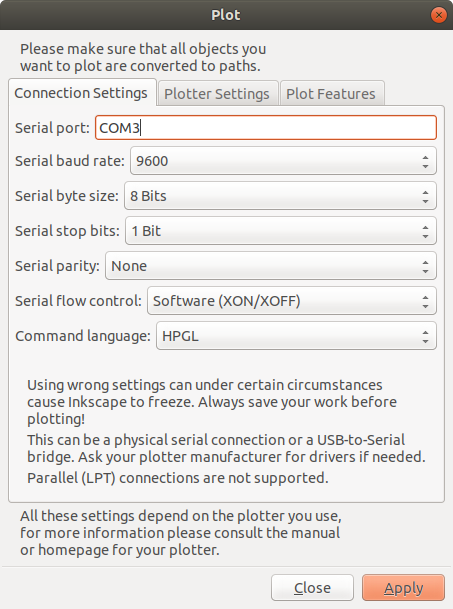
\includegraphics[width=0.45\textwidth]{images/connection_tab}
	}
	\hspace{0.05\textwidth}
	\subcaptionbox{Plotter Settings \label{fig:settings}}{
		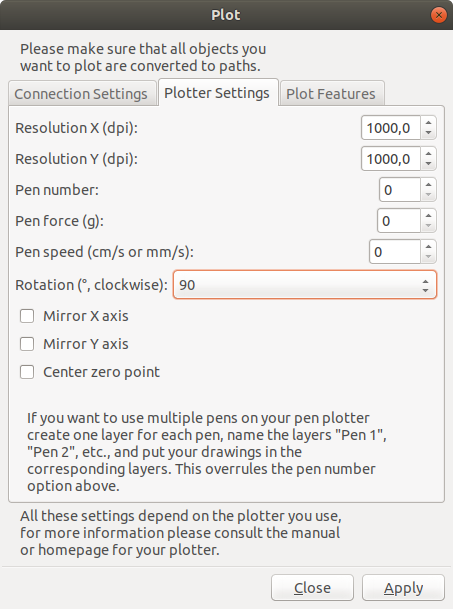
\includegraphics[width=0.45\textwidth]{images/plottersettings_tab}
	}
	\\
	\vspace{15pt}
	\subcaptionbox{Plot Features \label{fig:features}}{
		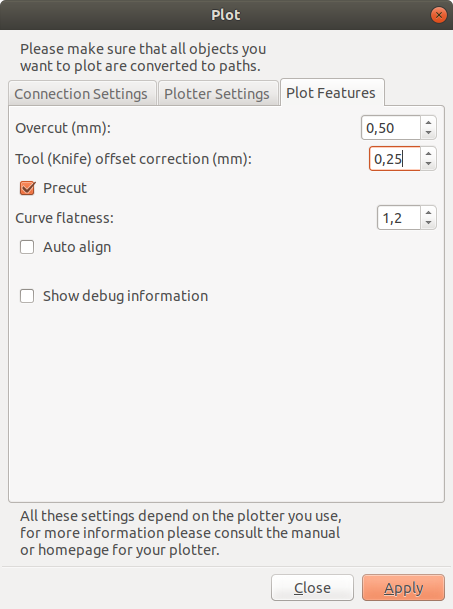
\includegraphics[width=0.45\textwidth]{images/plot_features_tab}
	}
\end{figure}

\chapter{Troubleshooting}
\section{Finding the correct serial port in Linux}
\label{sec:portLinux}
Connect the plotter and open a terminal. Switch to the directory \textit{/dev/} using
\begin{lstlisting}
cd /dev/
\end{lstlisting}
List all serial ports that are connected via USB:
\begin{lstlisting}
ls | grep ttyUSB
\end{lstlisting}
There should be one device named \textit{ttyUSB} with a number suffix, i.e. \textit{ttyUSB0}. Use this as the serial port in Inkscape as \textit{/dev/ttyUSB<Number>}, i.e. \textit{/dev/ttyUSB0}.

\section{Additional setup in Linux}
\label{sec:setupLinux}
If Inkscape cannot access the serial port you have to add the user running Inkscape (probably yourself) to the group \textit{dialout}:
\begin{lstlisting}
sudo adduser <username> dialout
\end{lstlisting}
In case Inkscape is telling you ”pySerial is not installed“, you have to install the corresponding package for your distribution. In Ubuntu this is \textit{python-serial}:
\begin{lstlisting}
sudo apt-get install python-serial
\end{lstlisting}

\section{Fixing the Inkscape plotting extension}
Without this fix the plotter will not lift the knife when returning to its origin after it has finished cutting, which will ruin your precious plot. We already applied this fix at the PC standing next to the laser cutter.

Open the Python script containing the plotting extension. In Windows this is \textit{C:\textbackslash Program Files\textbackslash Inkscape\textbackslash share\textbackslash extensions\textbackslash plotter.py}, in Linux it's \textit{/usr/share/inkscape/extensions/plotter.py}. Note: you need admin/root privilege in both Windows and Linux to edit this file.

Look for the last line in the function \lstinl{convertToHpgl()}. It should be somewhere around line 107:
\begin{lstlisting}
self.hpgl = hpglInit + self.hpgl + ';SP0;PU0,0;IN; '
\end{lstlisting}
Change this as follows and save the file.
\begin{lstlisting}
self.hpgl = hpglInit + self.hpgl + ';PU0,0;IN; '
\end{lstlisting}

\section{Fast blinking LED above \textit{Off-line}}
The plotter encountered an error. Press \textit{Reset} and set up speed, pressure and origin again. This might happen, when you are trying to plot outside the range of the knife. Shrink your object or move the material and origin.